\documentclass{article}

\usepackage{ipprocess}
%\usepackage{lmodern}
\usepackage{longtable}
\usepackage[utf8]{inputenc} 
\usepackage[T1]{fontenc}
\pagestyle{fancy}
\usepackage{libertine}
\usepackage{epstopdf}
\usepackage{rotating} % rotate table 90 degrees
\usepackage{pdflscape} % set ladscape/portrait pdf pages
\usepackage[table]{xcolor}

%\usepackage[author={João Carlos Nunes Bittencourt}]{pdfcomment}

%%%%
\definecolor{darkred}{rgb}{0.55,0.0,0.0}
%%%%

\sloppy

\graphicspath{{./pictures/}}
\makeindex
\begin{document}
%%%%%%%%%%%%%%%%%%%%%%%%%%%%%%%%%%%%%%%%%%%%%%%%%%
%% Building front cover
%%%%%%%%%%%%%%%%%%%%%%%%%%%%%%%%%%%%%%%%%%%%%%%%%%
\DocumentTitle{Plano de Verificação Funcional}
\Project{MUSA}
\Organization{Fazemos Qualquer Negócio Inc.}
\Version{Compilação 1.0}
% Make front cover
\capa

%%%%%%%%%%%%%%%%%%%%%%%%%%%%%%%%%%%%%%%%%%%%%%%%%%
%% Revision History
%%%%%%%%%%%%%%%%%%%%%%%%%%%%%%%%%%%%%%%%%%%%%%%%%%
  \section*{\center Histórico de Revisões}
  \vspace*{1cm}
  \begin{center} % aqui comeTBDa o ambiente tabela
    \begin{longtable}[pos]{|m{2cm} | m{7.2cm} | m{3.8cm}|} 
      \hline % este comando coloca uma linha na tabela
      \cellcolor[gray]{0.9}
      \textbf{Data} & \cellcolor[gray]{0.9}\textbf{Descrição} & \cellcolor[gray]{0.9}\textbf{Autor(es)}\\ \hline
      \hline
      \small 23/10/2014 & \small Criação do documento. & \small Terseu Hunter \\ \hline 
      \small 24/11/2014 & \small Refatoração do documento & \small Anderson Queiroz e Manuelle Macedo \\ \hline 
    \end{longtable}
  \end{center}

  \newpage
	%%%%%%%%%%%%%%%%%%%%%%%%%%%%%%%%%%%%%%%%%%%%%%%%%%	
	%% Place TOC
	%%%%%%%%%%%%%%%%%%%%%%%%%%%%%%%%%%%%%%%%%%%%%%%%%%  
  \tableofcontents
  \newpage

	%%%%%%%%%%%%%%%%%%%%%%%%%%%%%%%%%%%%%%%%%%%%%%%%%%
	%% Document Prelimiary Content
	%%%%%%%%%%%%%%%%%%%%%%%%%%%%%%%%%%%%%%%%%%%%%%%%%%
  \section{Introdução}

	\subsection{Propósito do Documento}
	O objetivo deste documento é definir o plano de verificação da implementação MUSA. Este documento inclui o ambiente de verificação utilizado para realizar a verificação do processador, ao lado das principais características do design, a lista de testes, lista de \textit{assertions} e outros.
	
	\subsection{Stakeholders}
  \FloatBarrier  
  \begin{table}[H] 
    \begin{center}
      \begin{tabular}[pos]{|m{5cm} | m{8cm}|} 
        \hline % este comando coloca uma linha na tabela
        \cellcolor[gray]{0.9}\textbf{Nome} & \cellcolor[gray]{0.9}\textbf{Papéis/Responsabilidades} \\ \hline
        Anderson, Manuelle e Weverson & Verificação Funcional \\ \hline
        Gabriel, Lucas, Mirela, Patrick, Vinicius e Tarles & Implementação \\ \hline
        Anderson e Manuelle & Analise \\ \hline       
      \end{tabular}
    \end{center}
  \end{table} 
  
  \subsection{Siglas e Abreviações}
  \FloatBarrier
  \begin{table}[H]
    \begin{center}
      \begin{tabular}[pos]{|m{2cm} | m{11cm}|} 
				\hline 
				\cellcolor[gray]{0.9}\textbf{Sigla} & \cellcolor[gray]{0.9}\textbf{Descrição} \\ \hline
				DUT		& Design Under Test \\ \hline
        IF    & Interface \\ \hline        
      \end{tabular}
    \end{center}
  \end{table}  

	%%%%%%%%%%%%%%%%%%%%%%%%%%%%%%%%%%%%%%%%%%%%%%%%%%
	%% Document Descrição
	%%%%%%%%%%%%%%%%%%%%%%%%%%%%%%%%%%%%%%%%%%%%%%%%%%
	\newpage
	\section{Visão Geral do DUT}
\begin{itemize}
\item Implementação de um plano de verificação.
\item Implementação de todos os testbenches necessários para o DUT completo e os DUTs
resultantes de hierarquização.
\item Implementação do DUT. Essa implementação é seguida pela simulação do DUV, juntamente
com o testbench.
\item Captação dos dados de simulação através da coleta dos itens de cobertura e dos logs
da simulação.
\item Análise da cobertura funcional, que pode levar a uma mudança de estímulos no
testbench e a uma nova simulação.
\end{itemize}

	
	\begin{figure}[H]
    	\centering
    	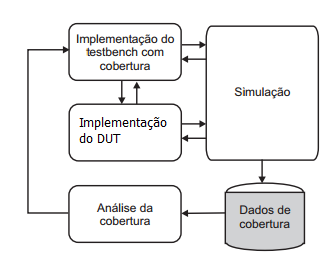
\includegraphics[width=.7\linewidth]{pictures/dutgeral.png}
  	\end{figure}
  	
	\newpage
	\section{Ambiente de Verificação}
	
  A metolologia de verificação adotada pelo projeto é baseada em \textit{testbench}, compondo parte das análises por meio de verificação baseada em \textit{waveform}. Situações especiais serão verificadas apartir de verificações baseadas em \textit{assertions}. A interface do DUT será responsável por coletar os dados do MUSA e enviá-los para o \textit{monitor}, no qual estarão declarados todos os \textit{assertions}. A Figura abaixo apresenta um modelo conceitual do ambiente de verificação.
		
	\begin{figure}[H]
    	\centering
    	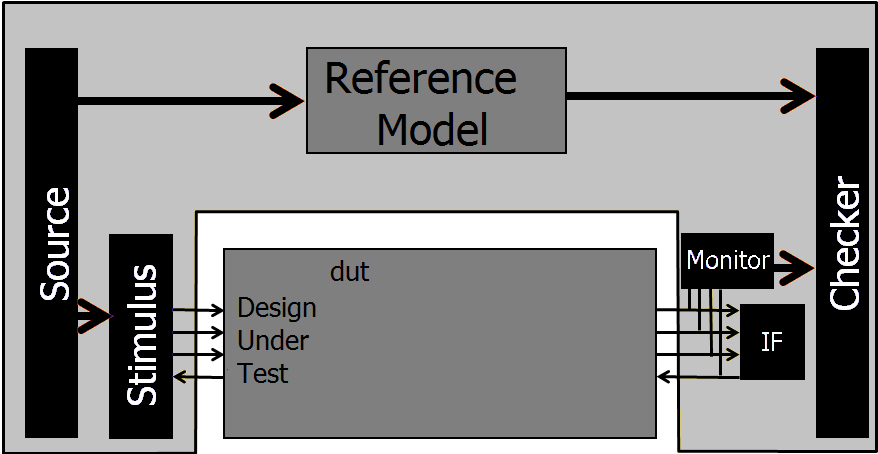
\includegraphics[width=.7\linewidth]{pictures/Diagrama.png}
  	\end{figure} 

	\subsection{Design Under Test Interface}
	
	O DUT IF promove a interface entre o \textit{monitor} e o DUT. Esta interface é responsável por controlar as informações trocadas entre o ambiente de verificação e o DUT. Dessa forma, ela deve conter instâncias de todos os sinais do DUT a serem utilizados ao longo do processo de verificação.
	
  A interface do DUT possui tabém a implementação dos \textit{assertions}. Estas estruturas têm como objetivo garantir que o comportamento dos sinais internos do DUT estão sendo produzidos e manipulados de maneira correta. Esta interface é instanciada na entidade \textit{top level} do ambiente de verificiação e seus sinais são conectados aos sinais provenientes do DUT.

	\subsection{Monitor e Checker}
	
  O \textit{monitor} é reponsável por observar o comportamento do DUT e coletar as suas saídas, de modo a verificar se as instruções estão funcionando da maneira desejada. O \textit{monitor} observa o comportamento dos sinais de controle e, quando necessário, captura os dados armazenados na memória de instruções e no banco de registradores.
	
  O \textit{checker} é responsável por executar o modelo de referência com o mesmo programa usado pelo DUT e comparar os dados armazenados na memória de dados e no banco de registradores. Se qualquer mal funcionamento for identificado, o \textit{checker} deve reportar uma mensagem de erro.

  Quando a execução do programa chega ao fim, o monitor deve invocar o \textit{checker}. O \textit{monitor} identifica o final da execução do programa a partir da instrução HALT.

	O teste que será executado no modelo de referência deve ser definido no arquivo \texttt{sim/tb/defines.sv}. Para executar o teste no DUT, o procedimento deve ser realizado no arquivo de memória de instruções \texttt{sim/tests/instrucoesMars.asm}, a partir da alteração do caminho especificado na funcão \texttt{read\_memh}.

	\subsection{Modelo de Referência}
  Tendo em vista garantir que o processador executará as instruções corretamente, foi desenvolvido um modelo de referência, capaz de simular o comportamento do processador MUSA. Este modelo é capaz de executar todas as instruções suportadas pelo MUSA. O arquivo do modelo de referência está localizado no diretório \texttt{sim/model/main2.c}.
	
	\subsection{Especificações de Projeto do Ambiente de Verificação}
  \FloatBarrier
    \begin{center}
			\rowcolors{1}{white}{gray!25}
      \begin{longtable}[pos]{| m{6cm} | m{8cm} |} \hline  
	      \rowcolor{black}
        \multicolumn{1}{|c|}{\textbf{\textcolor{white}{Componente}}} & 
        \multicolumn{1}{|c|}{\textbf{\textcolor{white}{Descrição}}} \\ \hline
        \endfirsthead
        \hline
        \multicolumn{2}{|l|}
        {{\bfseries continuação da página anterior}} \\
        \hline
        \rowcolor{black}
        \multicolumn{1}{|c|}{\textbf{\textcolor{white}{Componente}}} & 
        \multicolumn{1}{|c|}{\textbf{\textcolor{white}{Descrição}}} \\ \hline
        \endhead
        \hline \multicolumn{2}{|r|}{{continua na próxima página}} \\ \hline
        \endfoot

        \hline
        \endlastfoot
      	Nome do Documento         		          & Plano de Verificação do MUSA  	\\ \hline
      	Versão e data do documento 		          & Versão 1.0, 23 de outubro de 2014  	\\ \hline      	
      	Autor(es) / Proprietário(s) 		        & Terseu Hunter  	\\ \hline
      	Metodologia de Verificação	          	& Top-Down  	\\ \hline
      	Métodos de Verificação	          			& Simulation and Formal Verification  	\\ \hline
      	Aplicação   		          			        & ModelSim ALTERA Edition  	\\ \hline
      	Linguagens 		          			          & System Verilog  	\\ \hline
      	Ambiente de verificação   	            &	Custom testbench  \\ \hline	
      	Arquivos de teste				                &	No diretório: sim/tests \\ \hline
      	Tecnologias	                            &	FPGA Cyclone 3 Development Board  \\ \hline
      \end{longtable}
    \end{center}	
	
	\newpage
	\section{Lista de Funcionalidades}
	
  \FloatBarrier
    \begin{center}
			\rowcolors{1}{white}{gray!25} 
      \begin{longtable}[pos]{| c | m{9cm} | c |} \hline  %14cm
	      \rowcolor{black}
        \multicolumn{1}{|m{2cm}|}{\centering\textbf{\textcolor{white}{Feature Número}}} & 
        \multicolumn{1}{m{9cm}|}{\centering\textbf{\textcolor{white}{Feature Descrição}}} &
        \multicolumn{1}{c|}{\textbf{\textcolor{white}{Prioridade}}}  \\ \hline
        \endfirsthead
        \hline
        \multicolumn{3}{|l|}
        {{\bfseries continuação da página anterior}} \\
        \hline
        \rowcolor{black}
        \multicolumn{1}{|m{2cm}|}{\centering\textbf{\textcolor{white}{Feature Número}}} & 
        \multicolumn{1}{m{9cm}|}{\textbf{\textcolor{white}{Feature Descrição}}} &
        \multicolumn{1}{c|}{\textbf{\textcolor{white}{Prioridade}}}  \\ \hline
        \endhead
        \hline \multicolumn{3}{|r|}{{continua na próxima página}} \\ \hline
        \endfoot

        \hline
        \endlastfoot
      	MUSA\_F1      & Signal are activated based on the instruction.  &	10 \\ \hline   	
      	MUSA\_F2      & Communication with Instruction Memory &	9 \\ \hline
      	MUSA\_F3      & Read and write operation to the Data Memory. &	9 \\ \hline
      	MUSA\_F4      & Read and write operation to the Register File. &	10 \\ \hline
      	MUSA\_F5      & All interfaces protocols must work properly. &	9 \\ \hline     	
      \end{longtable}
    \end{center}	

\begin{landscape}		

\section{Lista de Testes}

  \FloatBarrier
    \begin{center}
			\rowcolors{1}{white}{gray!25} 
      \begin{longtable}[pos]{| c | m{5cm} | c | c | c | c | c | c |} \hline  %14cm
	      \rowcolor{black}
        \multicolumn{1}{|m{2cm}|}{\centering\textbf{\textcolor{white}{\mbox{Número} do Teste}}} & 
        \multicolumn{1}{m{5cm}|}{\centering\textbf{\textcolor{white}{Descrição}}} &
        \multicolumn{1}{c|}{\textbf{\textcolor{white}{Método}}} &
        \multicolumn{1}{c|}{\textbf{\textcolor{white}{Nível}}} &
        \multicolumn{1}{m{3.8cm}|}{\centering\textbf{\textcolor{white}{Funcionalidade \mbox{Verificadas}}}} &                
        \multicolumn{1}{c|}{\textbf{\textcolor{white}{Prioridade}}} & 
        \multicolumn{1}{c|}{\textbf{\textcolor{white}{Proprietário}}} &
        \multicolumn{1}{c|}{\textbf{\textcolor{white}{Situação}}} \\ \hline
        \endfirsthead
        \hline
        \multicolumn{8}{|l|}
        {{\bfseries continuação da página anterior}} \\
        \hline
        \rowcolor{black}
        \multicolumn{1}{|m{2cm}|}{\centering\textbf{\textcolor{white}{\mbox{Número} do Teste}}} & 
        \multicolumn{1}{m{5cm}|}{\centering\textbf{\textcolor{white}{Descrição}}} &
        \multicolumn{1}{c|}{\textbf{\textcolor{white}{Método}}} &
        \multicolumn{1}{c|}{\textbf{\textcolor{white}{Nível}}} &
        \multicolumn{1}{m{3.8cm}|}{\centering\textbf{\textcolor{white}{Funcionalidade \mbox{Verificadas}}}} &                
        \multicolumn{1}{c|}{\textbf{\textcolor{white}{Prioridade}}} & 
        \multicolumn{1}{c|}{\textbf{\textcolor{white}{Proprietário}}} &
        \multicolumn{1}{c|}{\textbf{\textcolor{white}{Situação}}} \\ \hline
        \endhead
        \hline \multicolumn{8}{|r|}{{continua na próxima página}} \\ \hline
        \endfoot

        \hline
        \endlastfoot
      	MUSA\_T1      & Execução de todas as instruções da categoria aritmética.          &	Sim       & Unit & MUSA\_F1, MUSA\_F4 & 5 & Anderson  & 70\% \\ \hline   
      	MUSA\_T2      & Execução de todas as instruções de transferência de dados.        &	Sim       & Unit & MUSA\_F1, MUSA\_F4 & 5 & Anderson  & 70\% \\ \hline   
      	MUSA\_T3      & Execução de todas as instruções da categoria lógica.              &	Sim       & Unit & MUSA\_F1, MUSA\_F4 & 5 & Anderson & 70\% \\ \hline  
      	MUSA\_T4      & Execução de todas as instruções da categoria salto condicional.   &	Sim       & Unit & MUSA\_F1, MUSA\_F4 & 5 & Anderson & 70\% \\ \hline 
      	MUSA\_T5      & Execução de todas as instruções da categoria salto incondicional. &	Sim       & Unit & MUSA\_F1, MUSA\_F2 & 5 & Anderson & 70\% \\ \hline 
	      MUSA\_T6      & Acesso à memória de declarados                                    &	Assertion & Unit & MUSA\_F3           & 7 & Manuelle e Weverson & 80\% \\ \hline        
	      MUSA\_T7      & Acesso à memória de instruções                                    &	Assertion & Unit & MUSA\_F4           & 9 & Manuelle e Weverson & 80\% \\ \hline        
	      MUSA\_T8      & Execução de programas completos sob a arquitetura.                &	Sim       & Unit & MUSA\_F3, MUSA\_F4 & 8 & Anderson, Manuelle e Weverson & 0\% \\ \hline        
	      MUSA\_T9      & Teste de todos os protocolos de interface.                        & Assertion & Unit & MUSA\_F5           & 8 & Anderson, Manuelle e Weverson & 0\% \\ \hline        

      \end{longtable}
    \end{center}		
  \end{landscape}
  
  \newpage
	\section{Assertions}

  \FloatBarrier
    \begin{center}
			\rowcolors{1}{white}{gray!25} 
      \begin{longtable}[pos]{| c | l | c |} \hline  %14cm
	      \rowcolor{black}
        \multicolumn{1}{|c|}{\textbf{\textcolor{white}{Número}}} & 
        \multicolumn{1}{m{10cm}|}{\centering\textbf{\textcolor{white}{Critério}}} &
        \multicolumn{1}{c|}{\textbf{\textcolor{white}{Status}}}  \\ \hline
        \endfirsthead
        \hline
        \multicolumn{3}{|l|}
        {{\bfseries continuação da página anterior}} \\
        \hline
        \rowcolor{black}
        \multicolumn{1}{|c|}{\textbf{\textcolor{white}{Número}}} & 
        \multicolumn{1}{m{10cm}|}{\centering\textbf{\textcolor{white}{Critério}}} &
        \multicolumn{1}{c|}{\textbf{\textcolor{white}{Status}}}  \\ \hline
        \endhead
        \hline \multicolumn{3}{|r|}{{continua na próxima página}} \\ \hline
        \endfoot

        \hline
        \endlastfoot
      	MUSA\_A1      & Assertion para a busca correta das instrução.            &	Em andamento \\ \hline   	
      	MUSA\_A2      & Assertion para verificar a operação de decodificação     &	Em andamento \\ \hline
      	MUSA\_A3      & Assertion para verificar a operação do bloco de execução.&	Em andamento \\ \hline      	
      	MUSA\_A4      & Assertion para leitura da memória de dados e write back. &	Em andamento \\ \hline      	
      	MUSA\_A5      & Assertion para branches e instruções de salto. 		       &	Em andamento \\ \hline      	
      	MUSA\_A6      & Assertion para verificar os protocolos de interface. 		 &	Em andamento \\ \hline      	
      \end{longtable}
    \end{center}		
  
  \newpage
	\section{Recursos Requirements}
  \FloatBarrier
    \begin{center}
			\rowcolors{4}{gray!25}{white} 
      \begin{longtable}[pos]{| l | c | c | c | c |} \hline  %14cm
	      \rowcolor{black}
        \multicolumn{1}{|c|}{\textbf{\textcolor{white}{Recursos}}} & 
        \multicolumn{1}{c|}{\centering\textbf{\textcolor{white}{Quantidade}}} &
        \multicolumn{1}{c|}{\centering\textbf{\textcolor{white}{Descrição}}} &
        \multicolumn{1}{c|}{\centering\textbf{\textcolor{white}{Início}}} &
        \multicolumn{1}{c|}{\textbf{\textcolor{white}{Duração}}} \\ \hline
        \endfirsthead
        \hline
        \multicolumn{5}{|l|}
        {{\bfseries continuação da página anterior}} \\
        \hline
        \rowcolor{black}
        \multicolumn{1}{|c|}{\textbf{\textcolor{white}{Recursos}}} & 
        \multicolumn{1}{c|}{\centering\textbf{\textcolor{white}{Quantidade}}} &
        \multicolumn{1}{c|}{\centering\textbf{\textcolor{white}{Descrição}}} &
        \multicolumn{1}{c|}{\centering\textbf{\textcolor{white}{Início}}} &
        \multicolumn{1}{c|}{\textbf{\textcolor{white}{Duração}}} \\ \hline
        \endhead
        \hline \multicolumn{5}{|r|}{{continua na próxima página}} \\ \hline
        \endfoot

        \hline
        \endlastfoot
        \rowcolor{gray}
				\textbf{Recursos de Engenharia}     & 		&										 	& 		 			&  \\ \hline   	
      	Engenheiro de Verificação  					& 3 &	Alunos                	& 10/11 	      & 15 dias \\ \hline   
      	\rowcolor{gray}
				\textbf{Recursos Computacionais}     			& 		&										 	& 		 			&  \\ \hline   
				Computador 														& 3 &	Intel i5                	& N.A. 	      & N.A. \\ \hline   
      	\rowcolor{gray}
				\textbf{Recursos de Software} 				& 		&										 	& 		 			&  \\ \hline   
				ALTERA Quartus 											& 1		& WEB Edition					& 10/11	      & 21 dias \\ \hline 				
				ALTERA ModelSIM		 									& 1		& ALTERA WEB Edition	& 	  14/11    & 21 dias \\ \hline 
      \end{longtable}
    \end{center}		
  
  \newpage
	\section{Cronograma}

  \FloatBarrier
    \begin{center}
			\rowcolors{4}{gray!25}{white} 
      \begin{longtable}[pos]{| l | c | c | m{6.5cm} | m{2cm} |} \hline  %14cm
	      \rowcolor{black}
        \multicolumn{1}{|c|}{\textbf{\textcolor{white}{Recursos}}} & 
        \multicolumn{1}{c|}{\centering\textbf{\textcolor{white}{Início}}} &
        \multicolumn{1}{c|}{\centering\textbf{\textcolor{white}{Duração}}} &
        \multicolumn{1}{m{6.5cm}|}{\centering\textbf{\textcolor{white}{Ação}}} &
        \multicolumn{1}{m{2cm}|}{\centering\textbf{\textcolor{white}{Recursos}}} \\ \hline
        \endfirsthead
        \hline
        \multicolumn{5}{|l|}
        {{\bfseries continuação da página anterior}} \\
        \hline
        \rowcolor{black}
        \multicolumn{1}{|c|}{\textbf{\textcolor{white}{Recursos}}} & 
        \multicolumn{1}{c|}{\centering\textbf{\textcolor{white}{Início}}} &
        \multicolumn{1}{c|}{\centering\textbf{\textcolor{white}{Duração}}} &
        \multicolumn{1}{m{6.5cm}|}{\centering\textbf{\textcolor{white}{Ação}}} &
        \multicolumn{1}{m{2cm}|}{\centering\textbf{\textcolor{white}{Recursos}}} \\ \hline
        \endhead
        \hline \multicolumn{5}{|r|}{{continua na próxima página}} \\ \hline
        \endfoot

        \hline
        \endlastfoot
      	TBD     					& TBD	&	TBD dias 	& Definam as tarefas nesta tabela :) 	& N/A \\ \hline


      \end{longtable}
    \end{center}	
		
	

\end{document}
